\documentclass[a4paper]{article}

% 引入各类的包
\usepackage{geometry}
% 定制目录
\usepackage{tocloft}
% 引入中文本地化的包,强制粗体(如果字体本身没有粗体,也显示粗体)
\usepackage[AutoFakeBold]{xeCJK}
% 设置间距的包(本文里面用的是行间距)
\usepackage{setspace}
% 首行进行indent的包
\usepackage{indentfirst}
% 引用
\usepackage{cite}
% 引用pdf,用在最后附录直接应用其他人的pdf
\usepackage{pdfpages}
% 图片编号
\usepackage{chngcntr}
% 启用目录链接
\usepackage{hyperref}
% 引入图片的库
\usepackage{graphicx}
% 页眉页脚设置的库
\usepackage{fancyhdr}


% 设置页边距
\geometry{left=3.17cm,right=3.17cm,top=2.54cm,bottom=2.54cm}
% 在数字序号前加“第”
\renewcommand{\cftsecpresnum}{第}
% 在数字序号后加“章”
\renewcommand{\cftsecaftersnum}{章}
% 设置数字序号区域的宽度
\setlength{\cftsecnumwidth}{5em}
% 让点变得密集
\renewcommand{\cftdotsep}{1}
% 设置宋体
\setCJKmainfont{SimSun}
% 设置英文字体
\setmainfont{Times New Roman}
% 设置黑体的名字为 hei
\setCJKfamilyfont{hei}{SimHei}
% 设置命令
\newcommand{\hei}{\CJKfamily{hei}}
% 第一个参数应该是图片,第二个参数指明是在哪个部分里面编号
\counterwithin{figure}{subsection}
% 链接的设置
\hypersetup{colorlinks,
	linkcolor=black,
	filecolor=black,
	urlcolor=blue,
	citecolor=black}

% 使其生效
\pagestyle{fancy}
% 详细设置
\chead{山东大学本科毕业论文}
\lhead{}
\rhead{}
% 重命名命令的名字
\renewcommand{\contentsname}{\centerline{目录}}
\renewcommand{\refname}{参考文献}
\renewcommand{\figurename}{图}
\renewcommand{\tablename}{表}
\renewcommand{\partname}{\centering{}}
% 创建俩个命令的名字
\newcommand{\enabstractname}{Abstract}
\newcommand{\cnabstractname}{中文摘要}
% 自定义字号
\newcommand{\小二}{\fontsize{18pt}{\baselineskip}\selectfont} 
\newcommand{\小三}{\fontsize{15pt}{\baselineskip}\selectfont}
\newcommand{\小四}{\fontsize{12pt}{\baselineskip}\selectfont}
% 自己设置一个中文摘要和英文摘要的环境
\newenvironment{enabstract}{
	\par
	\小四
	\noindent\mbox{}\hfill{\bfseries \小三 \enabstractname}\hfill\mbox{}
	\par
	\vskip 2.5ex}
{\par\vskip 2.5ex}
\newenvironment{cnabstract}{
	\par\小四
	\noindent\mbox{}\hfill
	{\bfseries \小三 \cnabstractname}
	\hfill\mbox{}
	\par
	\vskip 2.5ex
	}
{\par\vskip 2.5ex}
% 这个部分只是为了消除警告
\title{编译原理可视化课件}
\author{张琳}

\begin{document}

% 设置行间距为1.5
\setstretch{1.5}
% 在正文前的页码是大写罗马字
\pagenumbering{Roman}
% 设置字体,寻找更好的方法
\fontsize{12pt}{\baselineskip}\selectfont
\tableofcontents
% 目录与正文隔开
\newpage

% 从摘要开始的页码是阿拉伯数字
\pagenumbering{arabic}
\centerline{\textbf{\huge{\hei \小二 编译原理可视化课件的动画设计}}}
% 临时设置,应该包装起来会更合适
\vskip 2.5ex
\phantomsection
\begin{cnabstract}
	
编译原理是大学本科学习过程中的一门重要但难以掌握的一门学科。编译器
我们一般可以将其分成前端后端俩个部分,本科学习中主要学习了编译器中的前端部分。前端的内容在业界已经有很多成型的算法,不过学生在理解这些算法的时候,普遍存在着难以理解、容易混淆、形不成概念的问题,缺乏直观的认知,同时也会在细节的地方掌握不好。
		
这个课题的提出就是为了实现一个基于Web的可视化编译原理的课件,通过生动有趣的动画演示,实时的环境变量信息,清晰明了的算法步骤指示,将原本枯燥难以理解的课本内容,通过这些传达学生。这样有效解决学生学习枯燥无味的问题,增进学生学习编译原理的热情,也能够让老师更加容易指导学生学习。借助于web的力量,让任何人都可以在任何系统任何时刻都可以访问到这个系统,让学习更加方便无障碍。

\textbf{关键字:}编译原理、可视化、web系统、动画设计
\end{cnabstract}
\addcontentsline{toc}{section}{摘要}
\newpage

\phantomsection
\begin{enabstract}
Compiler theory is the college is very important and difficult to
master a course, it is divided into two parts front and back of
undergraduate study is mainly learning compiler front-end, but the
contents of the front end, although the industry has there are many
forming algorithm, but the students understand these algorithms time,
the prevalence of the problem is difficult to really learn, and in
most cases only a rough impression, but there is no intuitive
understanding and grasp of the details. The issue raised is to
implement a system that can effectively solve this problem visually,
but also try to stimulate students' enthusiasm for learning compiler
theory, so learning compiler theory is no longer boring .

\textbf{Keywords:} Compiler, Visualization, web system, animation design
\end{enabstract}
\addcontentsline{toc}{section}{Abstract}
\newpage


% 绪论
\section{引言}
\subsection{选题背景}
编译原理是在大学本科中非常重要的一门课,然而,它的难度也相对较大,虽然
说论起算法来说,并不如算法课那样高难,但是它具有工程意义上的复杂性,并
不能都用简介的算法来表述清楚,其工作原理很难被学生直观理解和掌握。而这
个选题的目的就是,制作一个可视化的编译原理课件,采用非传统展示类的工具
来制作这个可视化,而是使用崭新的 web 技术,通过背后强大的语言和各大类
库的支撑,能够实现一个既能展示丰富内容的编译过程可视化,又能够激发同学
主动参与学习过程的软件。
\subsection{选题目标}
\subsubsection{主要目标}
实现一个可以供学习编译原理课程的师生使用的基于web的可视化编译原理过程
的系统。其主体是一个web程序,可以运行在现代的浏览器上,并且也能通过现
代常用的包装方式,成为一个桌面上的本地程序甚至是手机上的APP,并且提供
一个可选的后台,用于保存学生的文法、老师的参考文法以及其他更多的内容。
选题的基本目标是,能够在这个系统上面进行一个简单的左递归消除、提取左公
因式、生成预测分析表、生成LL分析器,选题的最终目标是,实现编译原理课程
中所涉及的所有算法的可视化。而这之外的功能,属于选题的附属功能,是教学
实践中的最佳的补充,使得整个系统能更好融入日常教学系统,而不是作为一个
图形化工具的辅助存在。另一方面,选题的目标系统还应该具有可插拔的特点,
并不是指系统本身可以插拔新的内容,而是指的系统本身的各种实现,可以应用
于现有的教学系统中,这也就是说,系统的每一部分可以剥离出来,而成为其他
系统的组件,这样可以拓展选题的目标系统的可用性,减少重复的劳作。
\subsubsection{附属目标}
由于选题本身是一个应用型的课题,那么,文档就是一个很重要的部分,论文本
身并不能作为一个有效的文档,它只是论述了选题本身的内容。程序的文档我们
粗略分成了开发者文档与使用者文档。尽管我们在设计系统的时候,以我们的直
觉来使得这个系统使用起来符合学习计算机的师生的直觉,然而我们自己的使用
习惯与其他人的使用习惯并不能一致,因此我们需要产出一个使用说明书,用于
系统的使用说明。另一方面,我们还要使得这个系统得以长期维护下去,而不是
当我们团队在这个选题结束的时候,这个系统就已经失去了维护,那么它的价值
就变得非常有限。所以,我们还会准备一份开发者文档,用于叙述选题目标系统
的各个有价值的环节,论述选题目标系统的架构,使用的类库以及主要的设计思
想等等,这一部分内容在论文也有所体现,因此,论文本身也是一份供给开发
者参考的文献。
\subsection{技术背景}
\subsubsection{基础框架与开发工具}
我们进行的这个课题,选择了几个方面的框架,一方面是开发工具集的选择,我
们使用了 webstorm 作为我们首选的开发工具,配合一些辅助的开发工具,包括
git、node等等。而前端展示部分,使用了bootstrap作为基础的展示框架,而
angular作为逻辑安排的框架,另一方面,还使用了,typescript语言,而不直
接使用javascript语言,这一点是为了更好和后续的团队进行配合。

框架的选择有一定的随意性,这点体现在它局限在我们团队的认知上,我们团队
由于只有有限的时间以及有限的软件经验,因此能够认识到的框架的数量以及深
度有限,因此在课题中选择的框架具有一定的随意性。然而,框架的选择也是经
过我们团队慎重考虑过的,在我们长期的web开发中选择了这个框架。

之所以选择了这些工具,分别都有其背后的原因,主要围绕当前的团队开发效率,
未来的维护工作,作为课题的可行性,时间以及空间概念上的考虑。具体内容过
多,与课题本身的关系不如其他方面紧密,暂时不展开讨论。
\subsubsection{课题相关技术}
\paragraph{简述} 
现有的比较常见的作为对编译器前端的支持的软件有很多,比较著名的就有lex、
flex、Yacc、Bison等等,虽然这些提到的都只是支持生成c语言的词法分析器、
语法分析器,但是现实中还有很多其他语言的实现,在web中也有支持生成
javascript的实现。其实在课题的最初,应该要充分调查现在web技术中的相关
实现,如果有可能的话,把我们的课题的目标系统直接建立在其它的技术之上,
而不用自己从头开始写过。
\paragraph{动画设计}
动画设计方面,我们考虑了几个框架,最终决定使用 d3 作为我们写复杂动画的
框架,而使用 angular 中的 animate 模块来写一些简单的动画。d3 本身是一
个数据驱动的可视化类库,它具有非常强大的功能,而又不替用户做太多的事情,
不像其他的一些表格或者画图类的框架,本身规定了很多内容,所以无法产生灵
活多样的动画。d3 使用了 web 中的标准技术,只要在现代的浏览器上面就可以
运行,而不用依赖于一些特定的插件来完成动画,比如flash插件是不需要的。
而且,d3提供了非常好用的数据差异比较算法,可以让我们很好分工合作。一部
分人可以负责专门写好动画,根据数据的某些变化,然后写好画面应该如何发展,
而另一部分人可以专门负责写怎么样产生数据,在这俩者之间只需要把使用什么
样的数据这部分相当于协议,定好之后,就可以很方便进行模块之间的联系。除
此之外,d3中提供了大量辅助动画的函数,可以方便我们进行各类操作,而不用
重新去实现。而学习成本方面,在d3的官网有非常丰富的实例,各类的教程也很
多,包括中文的文档也比较全面,所以对比于其他的框架或者类库,d3在这部分
也是很有优势的。
\paragraph{词法分析器} 
lex或者flex作为词法分析器生成器,是在这个课题中我们自己去实现一个能满
足可视化展示的词法分析器的一个有效的参考,可以通过他们的源代码以及相关
的文档,来探索词法分析器在业界的实现。除此之外,因为他们本身是词法分析
器生成器,代码的思路必然和词法分析器有所区别,而他们生成的特定的词法分
析器也因为是生成代码,造成可读性并不好的问题。因此,还可以参考一些业界
手写的词法解析器作为参考,比如流行的浏览器核心的webkit中,就有对
javascript的词法解析器的代码。实际上,我们本身的系统主要的目的是易于理
解,所以主要的代码参考还是来自于编译原理书本上的内容。
词法分析器还需要演示关于有穷自动机与无穷自动机的内容,这些内容的演示我
们主要参考了网络上的一些现有的实现。
词法分析涉及到了正则表达、状态图,这些内容本身的知识量也比较大,但是在
大多数编译原理的课本中也只是介绍一部分他们的内容,更多的内容也在形式化
学习中才能学习到。这方面,一方面我们参考已有的词法分析器中的使用的正则
的情况,另一方面,我们参考一些专门介绍正则表达式、状态图的领域的书籍、
论文还有网络上面各类的博客。
\paragraph{语法分析器}
语法分析器是一个难点,虽然也是业界具有非常成熟的一系列算法,然而却也是
学生理解的困难点,另一方面,也有不少学生认为语法分析器能够被语法分析器
生成器所生成而不在意语法分析器的本身的原理,这在学习编译原理这门课中是
一种不利好的想法。实际上有Yacc和Bison作为主流的语法分析器生成器,而也
有大量大型的项目使用自己手写的语法分析器,这也证实了学习语法分析器的基
本原理是有利于理解现有的代码的。我们并没有完整实现语法分析器生成器,而
是,把语法分析器的几个步骤一一拆解出来,分别实现,并且辅助以不同的动画。
\subsubsection{测试技术}
在web的UI测试,其实在业界已经有比较成熟的方案,但是我们并没有采用自动化
UI测试的方案,而是选择了手工的UI测试。因为课题本身的系统还不方便进行自
动化的UI测试,而且系统界面本身比较没有很多的内容,手工测试即可满足要求。

对于逻辑方面的测试,我们使用了web开发中常见的测试框架,jasmine。它自身
包含了大量我们所需要的测试工具,包括expect、mock等等,其开发者团队开发
相当积极,在StackOverflow社区上面的问答数量也相当多,因此我们最终选择
使用这个测试框架进行测试。我们团队的成员也都是刚刚接触这个框架,但是已
经能很熟练使用这个框架进行测试。
% 需求与功能点
\section{需求和功能点}
这个部分详细论述了需求和功能点,为了给读者提供一个更全面的课题介绍。
\subsection{词法分析的动画设计}
\begin{itemize}
\item 词法分析动画设计,能够将词法单元、模式以及词素从动画上面说明清楚,
  能够实现适当的提示,包括鼠标移动上去的提示,本身的字幕提示以及任何其
  他合理的提示。
\item 输入缓冲动画设计,说明清楚缓冲的作用,在动画中要能够清晰标明指针
  的位置,缓冲区的特点,能够让用户自定义输入文本的内容,也能够提供从不
  同的地方输入文本的内容的功能,详细的要求参见对文法输入的要求。可以提
  供一定的算法步骤,进行算法演示,这部分可选,因为输入缓冲的目的是让同
  学理解输入缓冲,而输入缓冲的算法实践本身比较简单。
\item 词法单元的归约的动画设计,使用动画来说明词法单元归约的各种名词,
  即通过一个动画,展示串的各个部分分别指的是哪些内容,通过动画,来说明
  语言上的运算是怎么样子的。这里可以适当加上对正则匹配过程的动画演示,
  可以参考已有的开源项目,不一定做成动画,可以做成匹配过程可以看到的匹
  配元素,就已经能够比较清晰说明正则匹配的内容。
\item 词法单元的识别的动画设计,用一个动画,配合词素、词法单元名字、属
  性值的内容,来演示词法单元配合的时候应该如何去识别每一个词法单元,他
  们是怎么被标记出来的可以做出成动画,辅助一些流水线的效果。另外还需介
  绍基于状态转换图的词法分析的体系结构,这部分可以用动态的状态图来展示
  出来它的工作效果,可以辅以代码来查看当前执行的情况。
\item 有穷自动机的动画设计,这部分内容基础要求是通过算法步骤一步步展示
  如何进行子集构造,在这个基础上,应该能完成更高的目标,利用算法步骤得
  到的结果,来动态构造一个动态图。最后应该要点名字符串的算法效率,可以
  做一个在线的测试给出一个测试结果,让同学们能直观的理解字符串处理的效
  率。
\end{itemize}
\subsection{语法分析的动画设计}
\begin{itemize}
\item 语法分析树的动画设计,这部分不具体讲解算法,因此就展示任意给定的
  一段代码,再给定一个文法,展示下一个语法分析树的展开,预先应该存有多
  个代码段以及匹配的文法。而且,能够在一定范围内处理异常的情况,指的不
  是能修正错误,而是如果发生文法和代码不匹配的情况,能够告之用户这俩者
  之间有不匹配的情况,可以根据后面的算法,指明在匹配到哪里的时候出现错
  误。
\item 左递归消除的动画设计,这部分动画应该直接包括直接左递归和间接左递
  归的情况。能够用动画展示出来算法的每一步骤针对的是哪些元素,并且可以
  指示算法当前进行到的位置,以及可以停止获取当前的各项变量的情况。
\item 提取左公因子的动画设计,这个算法内容比较简单,动画可以按照算法的
  进程,演示每一个公因子被找到的过程以及被提取的过程。
\item FIRST和FOLLOW集合构造的动画设计,根据构造FIRST集和FOLLOW集的算法,
  依次计算每一个非终结符号的集合,可以以多个集合图的方式来演示动画,表
  现出如何找到这些集合的过程。
\item LL(1)文法的动画设计,对于这个文法,我们可以设计出一个简短的动
  画来说明它的内涵。另一个要求是做出它的预测分析表,用FIRST和FOLLOW集
  合来逐步构建一个,在动画中展示出,如何构建每一行每一列的元素,动画应
  与输入符号相关联的算法执行情况。可以设计出栈的动画,方便用户可以查看
  到进出栈的情况。
\item LR(0)语法分析的动画设计,展示自底向上的分析过程。
\item LR(1)语法分析的动画设计
\item LALR语法分析的动画设计
\end{itemize}
\subsection{文法管理}
\begin{itemize}
\item 支持从多种渠道输入文法,分别应该有直接输入文法,从文件中获取文法,
  从URL中获取文法,其中文件中获取文法应该支持直接拖拽来上传文法以及从
  文件管理器中选择文法这俩种方式。
\item 支持文法的保存与记录,可以对文法进行命名和归类,可以分享文法给其
  他人,可以对文法进行评注以及说明。
\item 支持对文法进行报错提示,指的是文法不符合既定的格式,具体的格式要
  求在程序内说明。
\item 
\end{itemize}
% 技术架构
\section{架构设计}
\subsection{基本情况}
课题目标系统是一个web系统,传统的后台是作为可选的部分存在,主要的应用
是前端,算法运行展示等等都不依托于后台,一部分数据的存储是依托于后台,
作为可选的组件,大多数用户需要的数据都在前端利用HTML5中相应的技术存放,
还可以通过另一个可选的组件,即包装这个web系统的桌面程序,存储到本地的
文件数据库中。
\subsection{具体架构}
\paragraph{前端逻辑结构} 系统的前端使用了 angular 来组织,利用了
angular中MVVM的架构特点,将前端系统模块化。在项目早期,我们几乎都是用
angular来组织代码,利用angular中的模块,利用angular中的各种成分,功能
构成了最终的系统。但是,angular新版本的出来,让我们意识到这种方式的局
限性,它局限于angular框架,而未来某一天我们可能会换掉这个框架,所以我
们借鉴了angular2的思路,使用了未来的标准模块化的方案。因为是来自于还没
有正式定下来的方案,我们加了一层转换器,也就是使用了一个新的语言
typescript。不过typescript没有增加我们的学习成本,在它上面基本上可以写
javascript,只是多了模块的概念。依靠这个模块和类,我们最终重构了我们的
项目,让现在的项目更容易看懂和测试。angular和typescript共同用于组织代
码,区别代码中的逻辑和视图。
\paragraph{前端界面} 而另一个我们采用的框架bootstrap则是帮我们处理基本
的浏览器兼容问题,并且提供给我们大量可以使用的web组件,便于我们最终创
造一个能在各种设备上面访问的web系统。而且bootstrap并不像其他的UI框架,
具有类似绑架的行为,将我们的系统绑架在他们上面,它本身具有相当开放的开
发方式,便于我们自己定制修改主题,甚至直接写其他的样式,而不用考虑怎么
和bootstrap进行配合。最重要的还有一块动画的部分,我们使用了D3作为一个
重要的展示类库。实际中,D3的帮助还显得不是很大,但是它确实在呈现各类图
标的时候,表现了它的能力。而作为候选,我们还可能直接操作canvas来进行,
如果后期需要更复杂的动画的情况下。D3允许我们通过操作数据,而它负责展示
动画,换句话说,只要我们改变了数据,就会产生相应的动画,其设计的思想和
我们在设计动画的时候,使用的思路是比较类似的。而且D3并不是自己负责给你
安排数据的展现方式,而是你可以设定数据进入移除更新的时候,分别需要采取
的动画形式。也就是说,D3只是帮助我们处理判断前后的数据有哪些不同,从而
应用不同的动画。不过,D3其实也帮助我们实现了很多常见的布局,比如可以很
方便用D3来写一些树状图、韦恩图等等,根据数据的结构,我们可以选择一个合
适的图来表达。
\paragraph{数据存储} 对于一部分的数据存储的需求,具体来说就是将用户输
入的文法进行存储、将生成的步骤序列进行存储、将生成的解析器进行存储等等
这部分需求,我们通过web中存储的API,存储在了浏览器中,从而,用户可以方
便获取这些数据,以便于用户不断重复操作来研究学习。如果用户希望可以把这
些数据存储到服务器中,我们也提供了一个可选的后端,通过后端,用户可以将
数据存储起来,方便自己在各个设备中都可以访问到这些数据。
\paragraph{本地应用}我们还采用了一个名为electron的框架,用于将web程序
封装成本地程序,这个组件可以用在用户没有合适的浏览器可以访问的情况下,
或者用户想要用有更好的浏览体验的时候,可以使用这个组件。通过electron,
我们可以生成不同平台的本地程序提供给用户使用。基于这个组件,我们还可以
拓展这个系统的功能,但是这部分扩展暂时不在计划之内,这里只是说明了一下
它可以做更多web平台可能目前无法做到的事情。
\paragraph{手机扩展}因为采用了angular,所以还有一个可能的扩展是,可以
通过ionic等框架,将应用延伸到手机端,而不需要写额外的代码。这其实有一
个前提,就是设计界面的时候考虑到手机屏幕的问题 ,而我们的界面目前还没
有考虑多少手机操作的问题,这部分内容也属于这个课题目标之外的设想。
\paragraph{后台及前后台交互} 一个可选的后台实际上是由express编写的,处
理一些简单的请求,将对应的数据存储到一个服务器端的文件数据库中,这部分
内容很简单,可以根据更具体的需求进行定制,目前我们只是预想了这部分需求,
并没有更实质性的计划。也就是说,后台的语言并没有局限在某种特定的语言,
也没有局限在特定的框架上面。但是已经考虑到这种想法,所以前台也会避免使
用一些会有冲突的解决方案。
% 动画设计
\section{动画设计}
\subsection{动画的表现形式}
对于现在常见的几种语法分析器,动画的形式基本围绕表格的方式进行,这实际
上包括个俩部分内容。一部分是,算法步骤,另一 部分是生成的分析表。动画将
算法步骤一步一步标出,提示当前的算法进行的信息,同时,在分析表处给出当
前分析表的执行情况。这基本上是传统的形式,也是我们手工进行分析的时候常
用的形式。在程序中,我们还会用生动的动画来体现变量之间的关系,比如利用
圆球包裹着变量的跳跃来体现变量之间的变化,还可以通过一些常见的树状结构、
维恩图结构、曲线图等等,来体现这点变化。动画的表现形式不应该局限于表格,
但是首先得有表格这样的东西来表达清晰的变量,然后再借助丰富的表现手段来
构造更形象的表达。
\begin{figure}
\centering

\includegraphics[width=0.7\linewidth]{img/recursive.jpg}
\caption{左递归消除,图中标记出将会改变的元素}
\label{fig:recursive.jpg}
\end{figure}
\subsection{动画设计的基本要求}
尽管在当今的社会中,可视化技术发展很迅猛,参与可视化工作的人们把动画做
得越来越绚丽多彩,然而可视化重要的一个部分,不是将动画写得有多么绚丽,
而是,动画能够让看到动画的人,真正感受到动画背后的深意,比如数据,比如
算法。在这个课题中,动画的目的是为了让教师能够更轻松教懂学生如何理解编
译原理过程中的各个算法,而学生也应该能够自己从动画中,相较于枯燥的文字,
静态的幻灯片,这些传统的内容中解脱出来,投入到一个更新鲜有趣的学习环境
中,利用这些有趣的动画,更容易更深刻理解算法,甚至可以透过这些动画,来
了解深一层次的算法含义。除了这个已经变得流行起来的可视化基本理念,我们
在设计中,还融入的,应该让学生能够自己去控制动画的过程,从而从动画的角
度来理解算法的运作。
\subsection{设计的几类动画}
动画中有纯粹展示类型的动画,比如其中的一个左递归消除的动画,它实现了按
步骤完成的整体动画,也提供了可以供用户单步进行的动画,用户也能够回退已
经执行过的动画,这些都在系统中实现了,但是,用户不能再动画运行过程中干
预动画的内容,也就是,它是一个纯粹的动画,甚至我们实现中就是将这个动画
对应的算法执行完毕之后,才开始进行动画,也就是说,动画的步骤是被实现记
录好了。
然而,系统中,并不只有这种类型的动画,另外也设计了一种动画,这种动画实
际上能够让用户参与进来,也就是说,用户可以改变某些变量,从而得到一个完
全不一样的动画形态,换句话说,用户不止可以在一开始的时候指定状态,甚至
可以在动画进行的过程中指定状态,从而让动画往不一样的方向发展。
根据动画的形态来区分系统中存在的动画,有这几种,分别是,形象化表达的动
画,比如消除左递归中,分别出现原本的产生式,接着,产生式的一部分被移除
画面,另一部分保留在画面中,并且缩进成一个紧凑的形态,这之后,,这个紧
凑的形态,再次伸展开来,插入新的字符,从而得到了产生式A,而此后,这个
产生式A再次消失。这个动画结束以后,再浮现出新的一组产生式,这组产生式
的字符就由刚才最先被移除的那部分字符组成,然后,再附上新的字符,使得产
生式消除左递归的过程得到充分地展现。
\subsection{如何设计这些动画}
要理解这些动画是如何设计出来的,那么需要先理解状态机是如何工作的,我们
在设计动画的时候,是把动画的表现抽离出来的,也就是,并不是将动画放入我
们所编写的算法中,而是作为独立的模块存在的,它算法本身的实现,几乎没有
什么联系,除了算法本身的特点将影响我们所采用的动画这一点以外。算法本身
运行的时候,自身是一个状态机,也就是,它从一个状态进入到另一个状态,或
者也可以回去,等等,并不与外界产生交互。然而,我们在外界是可以控制算法
是如何运行的。而之后,我们提取状态机,也就是算法,运行过程中,是如何改
变状态的,把这些状态的改变都记录下来,而最终就是根据这些状态的改变来生
成动画的。对于那种动画进行过程中,却可以改变算法的状态的,其实就是利用
了,状态机本身不对外界产生影响,但是,外界却能够对状态机产生影响这个道
理。而且,因为状态机记录的内容并不会丢失掉,不会因为算法重新执行到哪一
个而导致之前的步骤消失,所有的步骤都被完整记录下来。当外界去改变状态机
的一些状态走向的时候,也只是改变状态机未来的状态,也就是说,状态机还没
有走过的状态,所以不用担心状态丢失而不能有效表达动画。从这个层面上看,
这类型的动画,就不是离线的,而是实时的,围绕着用户的交互而进行的一种动
画。
除了状态机这样的观点来做动画以外,我其实更喜欢把算法看做是一系列的动作
制定器,在算法运行的时候,在程序的一些关键点中,加入算法记录函数,也就
是算法记录点,在这些算法记录点中,我可以提取动画所需要的数据,之后通过
获取这些算法记录点,我们可以将动画展示出来。当然,这样子实现的动画,是
没有额外的交互功能的,所谓额外交互功能就是除了单点执行中的前进后退,完
整执行一段动画这俩个主要的动能以外,没有别的交互功能。当然,如果暴露出
更多的信息,通过这些算法记录点,那么还可以让用户观测到这个算法执行到当
前时间段的时候,所有当前的变量信息、环境信息等等。这种方式,实际上就是
我们初次版本所要实现的方式,而更理想的状态机的方式,其实也是在这种方式
上面进行改造的结果。然而,在实现时,状态机的方式还有更多的问题需要解决,
所以在后续的开发中,我们要逐一解决这些问题。
\subsection{动画交互的要点}
\paragraph{动画交互}
动画交互需要注意分出来,哪一些是必要的部分,而哪一些是不必要的信息。还
有哪一些是要一直强调的部分,哪一些是在用户需要的时候才展现给用户看的部
分。具体来说的话,就是指的,在动画演示的过程中,有一些部分,要着重强调
出来,比如说,算法执行的主要步骤,算法在某一个时刻,实际上是对什么进行
操作,做了哪些操作,如果有办法,甚至还要体现为什么要做这些操作,让学生
可以通过看到这些动画,就能明白这些操作的含义,可以自己去完成这些操作。
除此之外,还有一些部分是在算法演示中不一定被强调的,比如当前执行的循环
次数,当前某个变量的值,这些东西的存在,可能会干扰学生进行感性的思考,
但是这些东西也必须存在,如果因为为了美观和可读性而直接牺牲了这些数据,
那么得到的内容是不完整的。当学生想要深入思考这些变量的变化的时候,就需
要这些更细节的内容,只是依靠图上的变化,是不足以让学生了解这些细节的变
化。

% 测试
\section{实现与测试}
\subsection{总体实现}
最终完成的部分有一个网页程序和一个本地程序,内容是同样的一个网页。均可
以通过按照需求描述的各种方法录入文法,并且可以将文法保存起来,而无需多
次重复输入文法。当前的实现中,缺少对词法分析的动画的支持,而实现了语法
分析动画的支持。
\subsection{使用}
用户首先需要下载这个程序,直接打开对应的网页或者本地程序,即可以使用,
另一种方式是将网页部署到服务器上面,然后打开对应的链接开始使用这个程序。

用户首先需要输入文法,通过文件上传拖拽或者是直接输入都可以。之后就可以
按照流程进行,分别是左递归消除、提取公因式、然后生成分析表,最后可以拿
着分析表分析用户输入的字符串。

在这些过程中,用户都可以通过控制栏来查看动画演示、算法步骤演示,在演示
过程中不能再更改相关的数据,而用户可以进行前进后退,而不仅仅只是往前看
动画演示。在界面的相应位置,用户可以看到当前的状态显示是如何的。用户还
可以将演示结果保存下来或者打印出来,生成相应的报告。

用户还可以将状态保存起来,下次打开程序的时候(网页或者本地程序)都可以
恢复到特定的状态,而无需重新调整到对应的状态。
\begin{figure}[!htb]
	\centering
	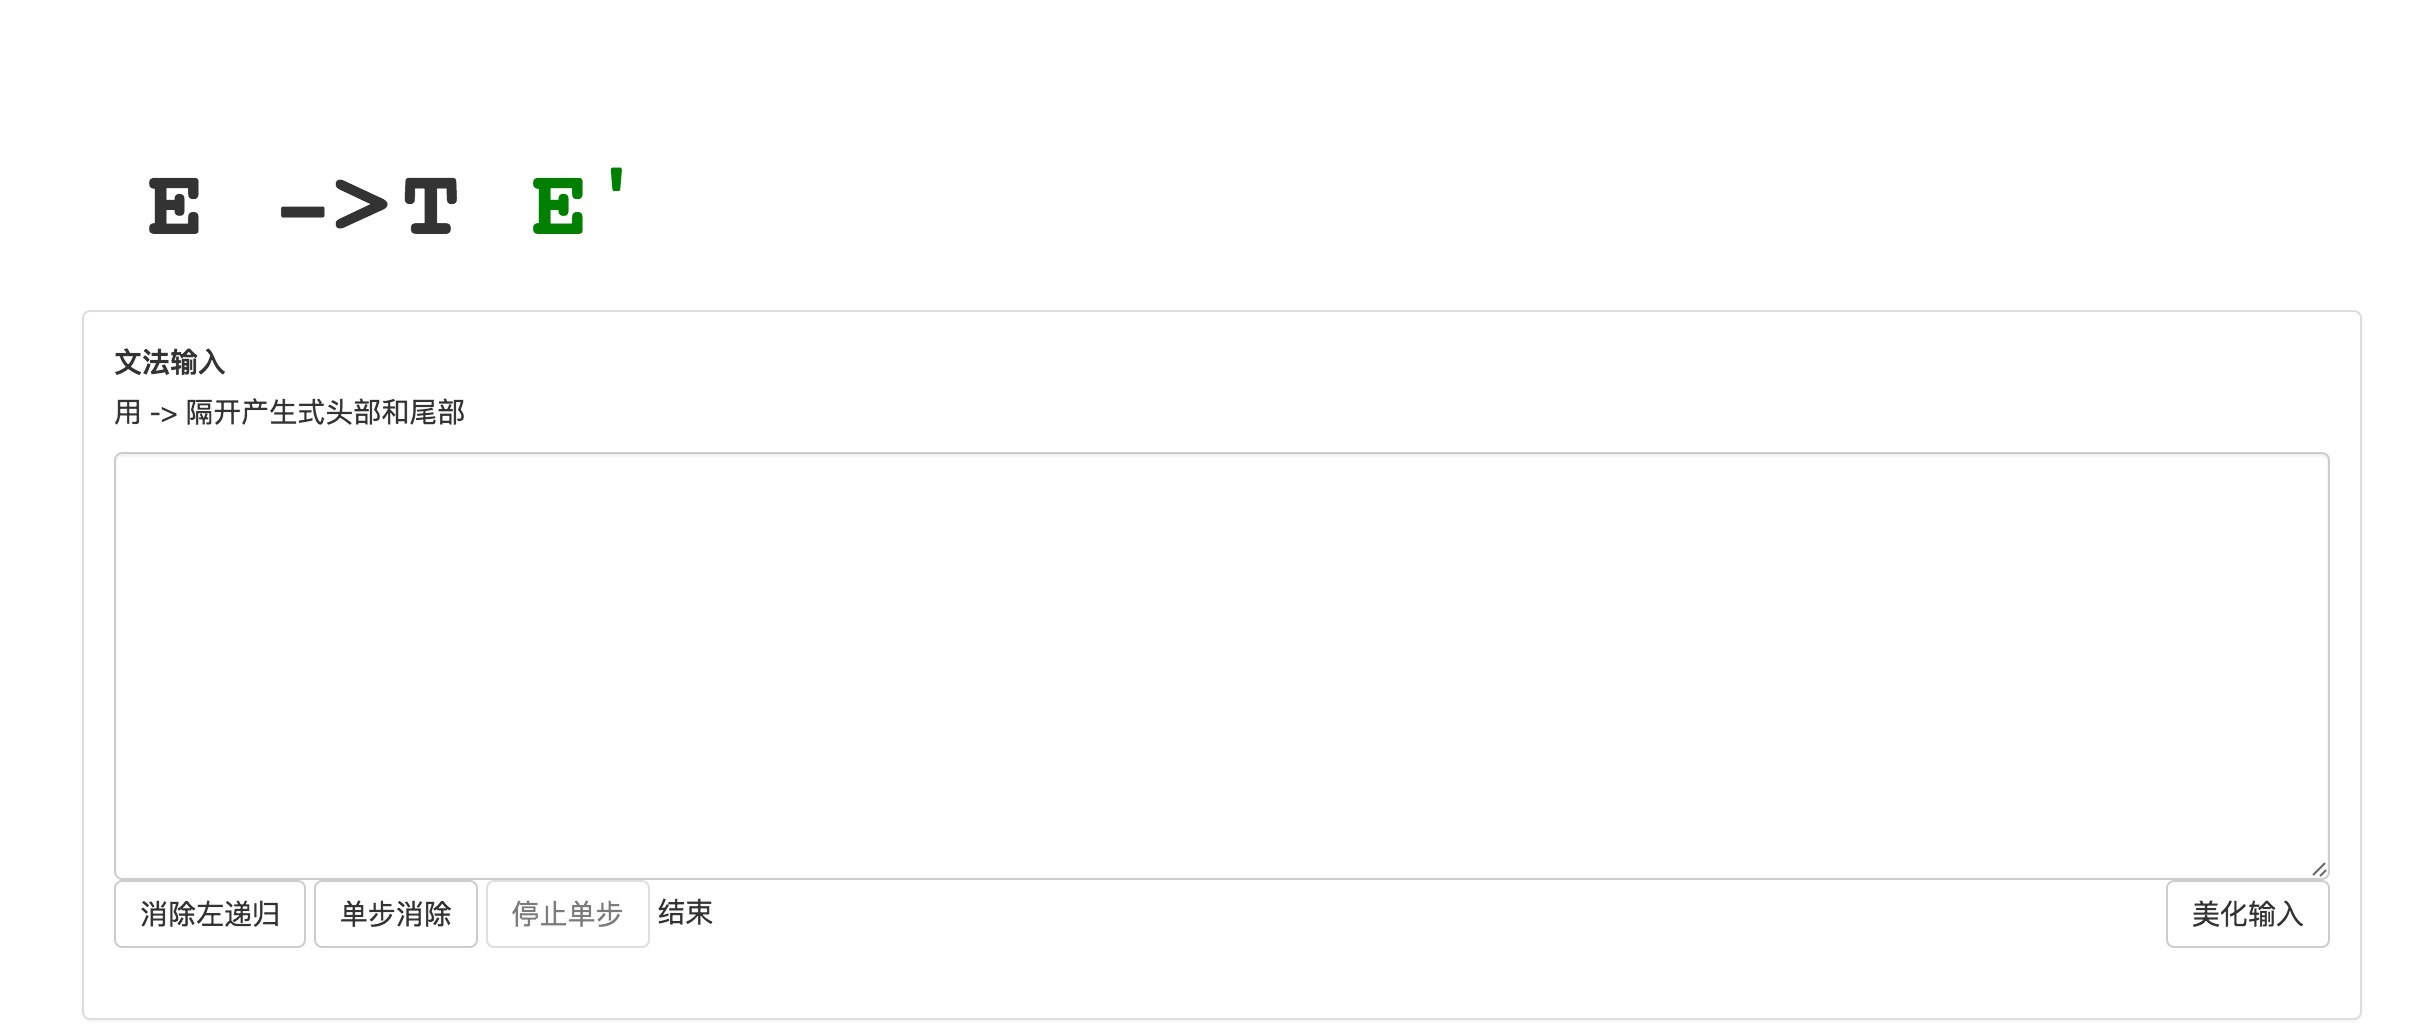
\includegraphics[width=1\linewidth]{img/grammarinput2.jpg}
	\caption{输入文法的初版}
	\label{fig:grammarinput2.jpg}
\end{figure}

\begin{figure}[!htb]
	\centering
	
\includegraphics[width=1\linewidth]{img/grammarinput3.jpg}
	\caption{输入文法,可以通过多种方式载入文法}
	\label{fig:grammarinput3.jpg}
\end{figure}

\begin{figure}[!htb]
	\centering
	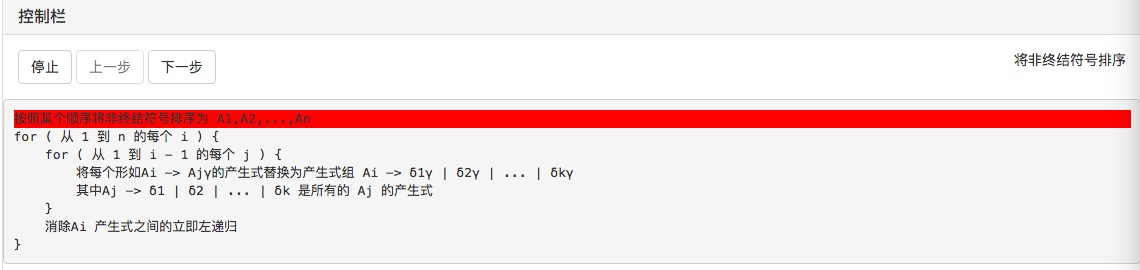
\includegraphics[width=1\linewidth]{img/leftrecursive2.png}
	\caption{左递归消除的算法步骤演示部分}
	\label{fig:leftrecursive2.png}
\end{figure}

\begin{figure}[!htb]
	\centering
	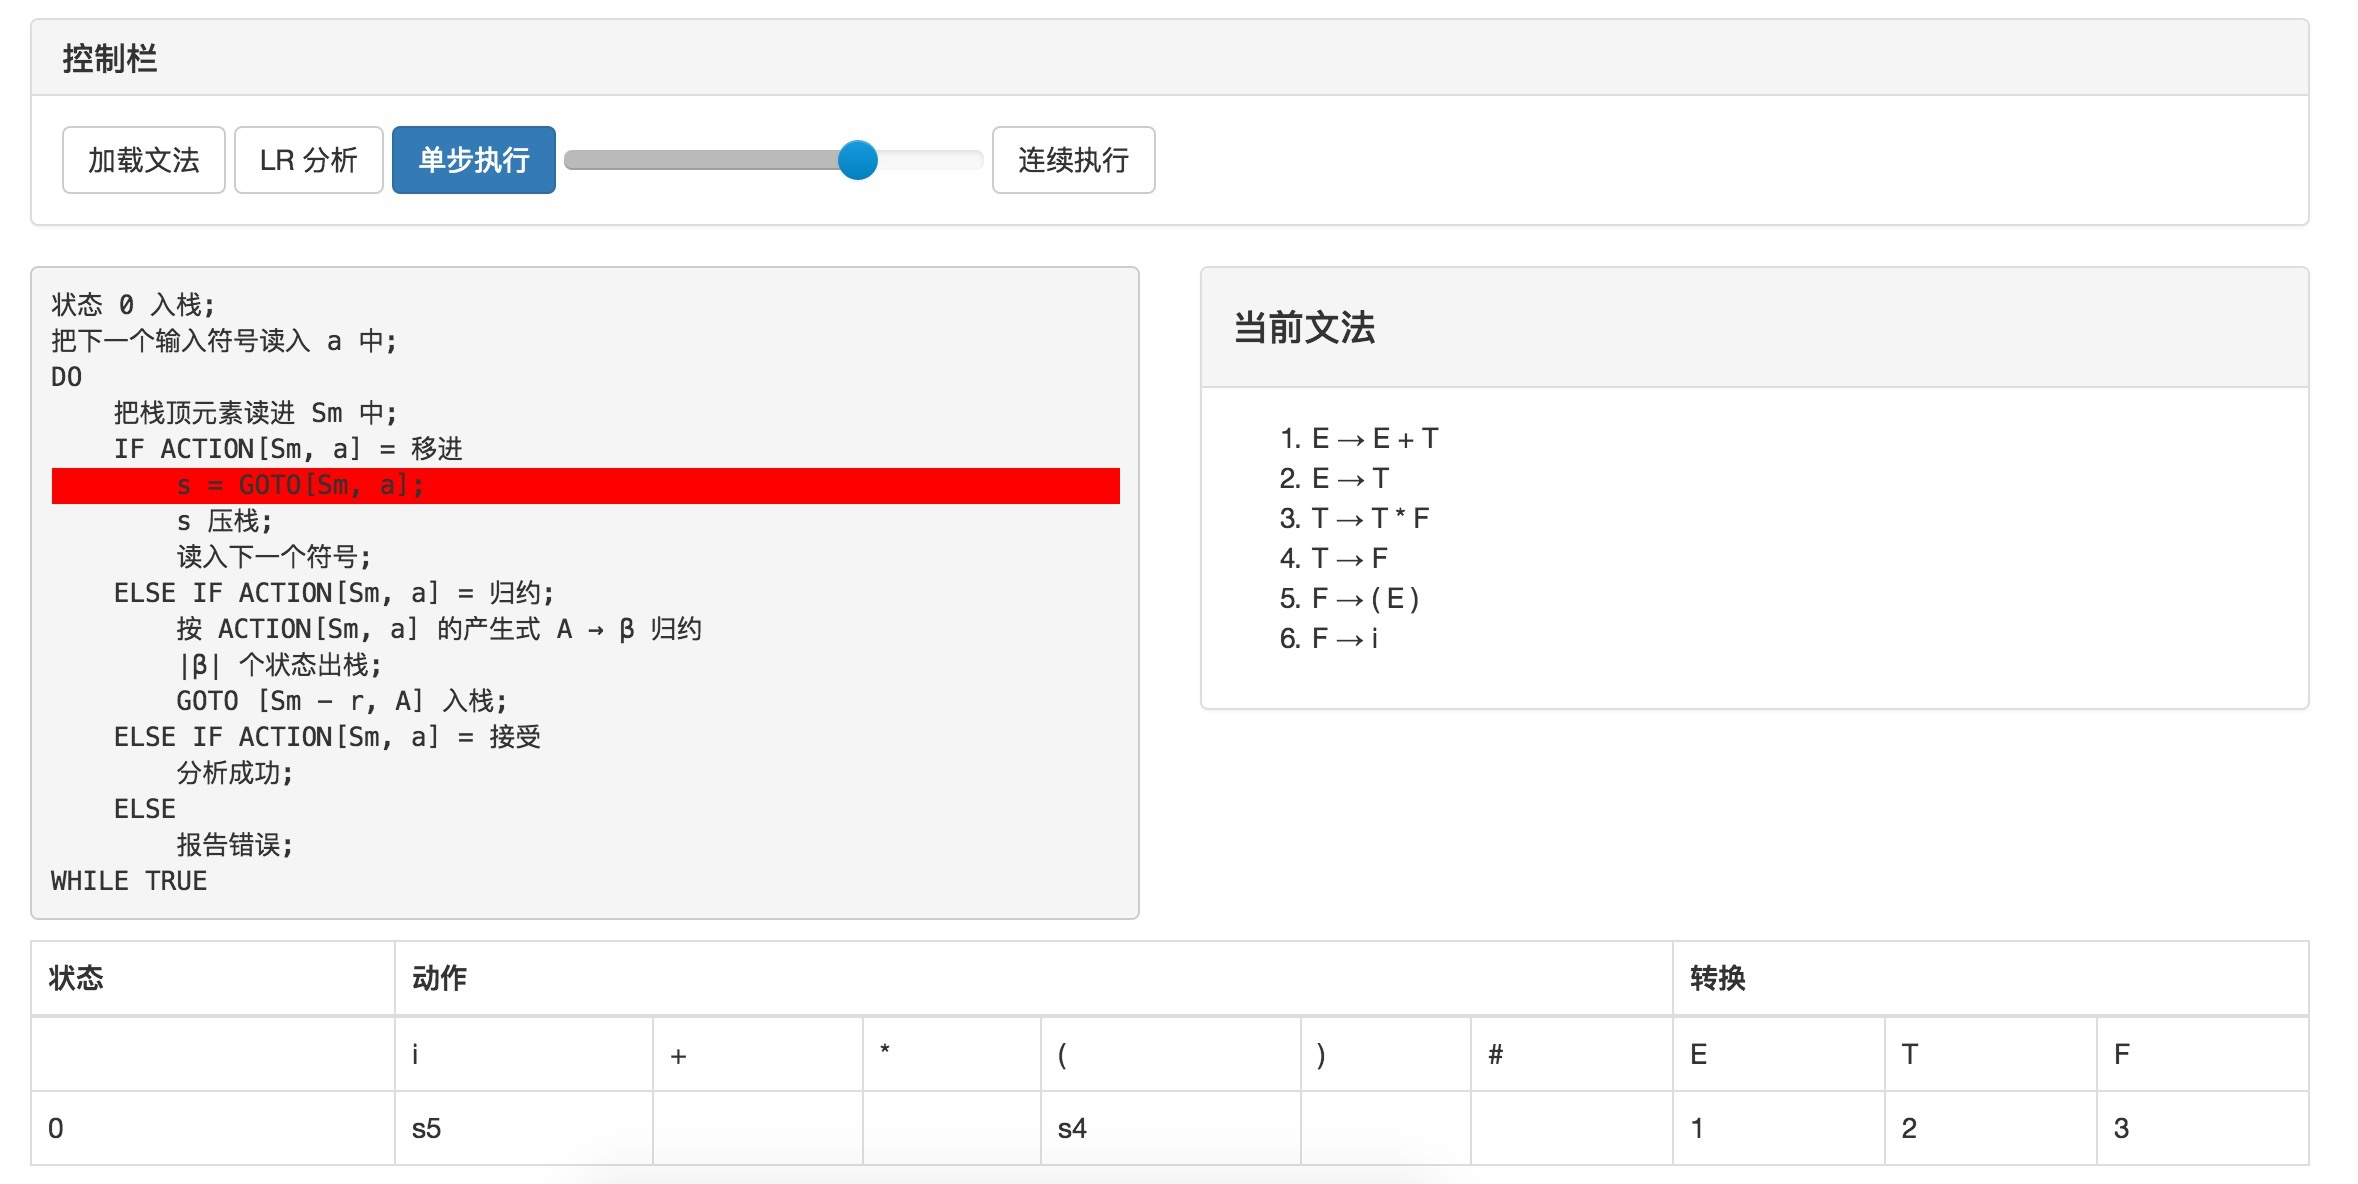
\includegraphics[width=1\linewidth]{img/tableanalyze.jpg}
	\caption{预测分析表的算法步骤演示部分}
	\label{fig:tableanalyze.jpg}
\end{figure}

\begin{figure}[!htb]
	\centering
	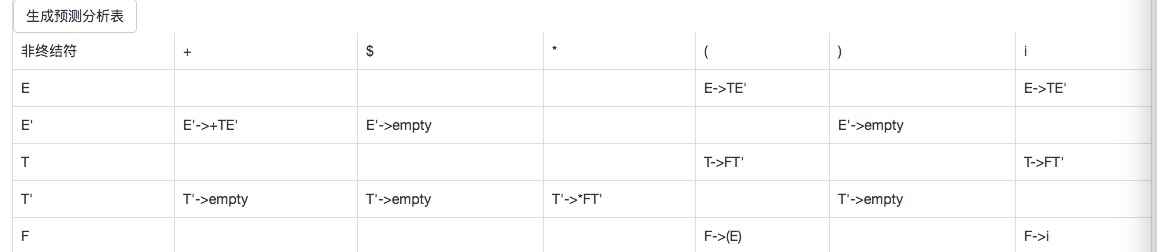
\includegraphics[width=1\linewidth]{img/table.png}
	\caption{预测分析表}
	\label{fig:table.png}
\end{figure}

\begin{figure}[!htb]
	\centering
	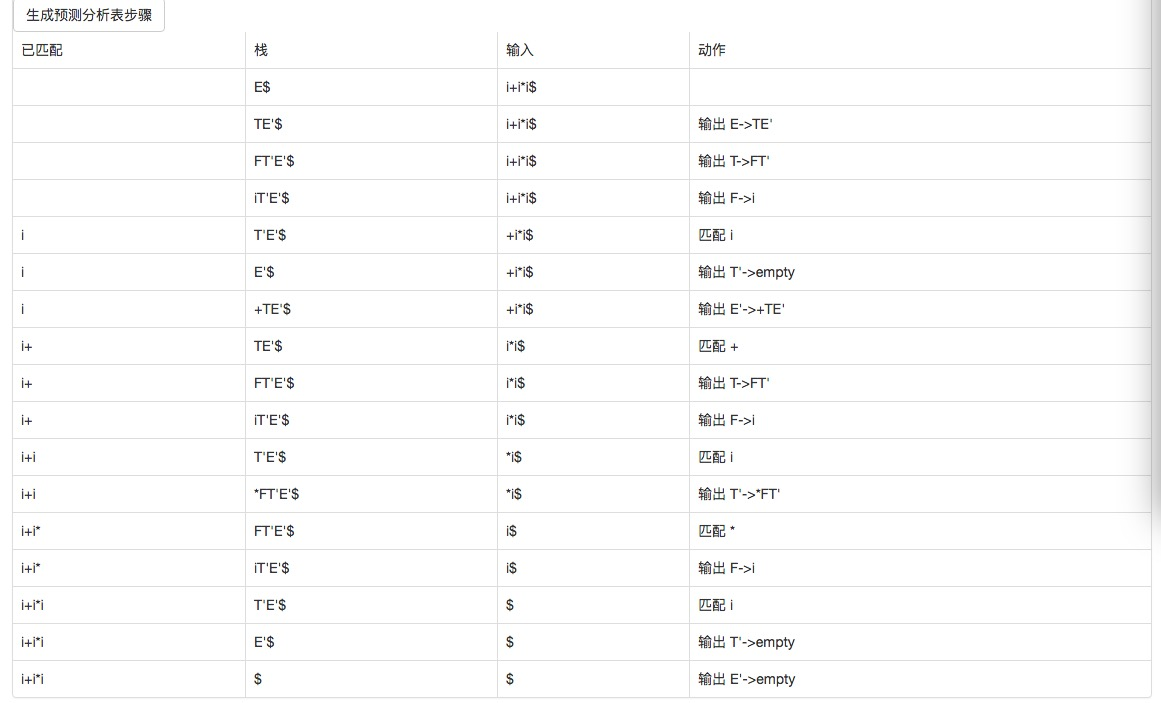
\includegraphics[width=1\linewidth]{img/tablegenerator.png}
	\caption{预测分析表执行步骤演示部分}
	\label{fig:tablegenerator.png}
\end{figure}

\subsection{界面测试}
界面主要是通过手工进行测试,相关的工具也有很多,但是考虑到系统的复杂性,
到目前的阶段还不需要引入专门的界面测试。而手工测试,主要集中在一下几方
面,分别是交互性测试,用来判断交互是否符合逻辑,是否存在错误的交互方法,
是否有交互的缺陷,兼容性测试,主要是针对不同浏览器的显示情况进行测试,
这部分测试我们不是很看重,能在大多数主流浏览器上能够运行即可,界面元素
和预想的偏差都不用在意,因为我们主要的目标平台是固定的浏览器,特别是,
我们可以要求用户安装特定的浏览器。还有其他的界面测试,比如界面的稳定性
测试,指的是在程序运行的时候,界面会不会卡顿,会不会出现一些不稳定的抖
动现象,会不会有一些不良的图像噪音,动画过程是否流畅等等。
\subsection{单元测试}
对于单元测试,我们将程序重构成由一个一个类组成的模块的时候,单元测试就
已经变得容易起来了。特别是,我们之后还严格控制了,底层逻辑的部分是不会
直接访问界面的元素,保证所有非界面相关的类都不会直接和界面联系,这便于
我们单独测试下面的每一个模块。实际测试的时候,我们将不同的模块分别测试,
对其调用相应的方法,并且和我们认定是正确的结果进行比对。单元测试除了验
证了我们本身程序代码是否符合预期的结果,还顺便推进了我们对代码的重构,
使代码变得更加清晰合理,有效避免了代码出现一团粥的情况,也有利于后来者
对代码的维护。
\subsection{算法测试}
算法测试本来是单元测试中的一种特例,然而由于其特殊性,这里单独拿出来讨
论。算法测试也需要满足单元测试的要求,给定多组的输入,都能得到正确或者
不正确的结果,只要是在预期的范围内,就是属于通过的测试。它不同于单元测
试的一点在于,我们有可能假设的预期就是错误的,所以,算法测试我们还需要
考虑这个算法是否真正解决了我们需要解决的问题,而不仅仅是得到了我们预期
的运行结果。
\subsection{系统测试}
有了其他的测试后之后,系统测试变得相对不关键,但是作为总体的一个测试环
节,我们也需要认真对待。对于整个系统的运作,其实不单单是把各个模块组合
起来,查看他们之间的联系是否正确,接口是否匹配,还需要查看不同模块之间
构成的系统,有没有把一些问题方法,比如性能问题是不是被放大,不兼容问题
是不是更严重了等等,这里面很多问题在单个模块的时候是可以在接受范围内的,
但是组装之后可能会出现更多的问题或者将问题放大,这些都是系统测试要做的
事情。除此之外,系统测试还将其他较为简单的测试也融入进来,比如安装测试,
验收测试等等,这些测试都归到系统测试中,由我们统一安排进行测试,保证这
个系统最终的可用性稳定性都能达到一定的高度。

% 总结
\section{疏漏与总结}
\subsection{代码复用}
在课题刚开始的时候,准备工作并不仅仅是学习,而应该是去看看已有的相关类
似的开源项目。在代码编写的时候,我们本应该尽可能利用已有的工具来完成一
些功能,虽然我们确实已经借助了一些开源工具来完成整个不属于我课题本身的
内容,比如使用了D3来完成动画,使用了angular以及typescript来组织整体的代
码。这些远远不够,只是在基础的框架上面打转,我们没有一开始就从其他的编
译器解析相关的项目入手,比如网络上已经存在的jison这样的开源项目,这是一
个很大的遗憾。如果能够更早意识到利用jison已经实现的算法,配合我们做动画
的思路,我们就可以更加专注于动画的设计上面,从而设计出更多更合理更吸引
人的动画。为什么这么说呢,算法本身就是很多人都已经实现了,课题的重心并
不是去重新实现这些算法,而是将这些算法可视化展现出来,然而最终我们却浪
费了大量的时间和精力去学习这些算法,重新实现这些算法。
\subsection{项目结构}
在程序设计的时候,因为想尝试更多的组织方式,所以中间有段时间去使用了更
新的一些开源类库,然而效果并不好。而在后来的实践中发现,在现有的基础上
去改变代码的结构,而不是通过替换底层我们依赖的框架,有时候的表现更好。
例如说,我们最后将代码使用 typescript 整理起来,依靠类与模块来把代码一
个一个独立出来,得到一个相对清晰的代码结构。当然,在界面展示那个层次上,
代码的可读性还不是那么好,但是我们相信,这些内容可以在后续不断改进中,
把他们处理得当。
\subsection{前人的研究}
我们在进行这项课题的研究的时候,忽略了其实导师教导过我们的事情,就是
着手开始一个课题的时候,要去先找找历史上,其他人对这个课题或者说是类似
课题的研究。这一步被我们省略了,或者是完全没有在一开始的时候意识到,这
是一个非常重要的疏漏。最后在整理论文的时候,其实我们已经看到了很多其他
科研人员研究的内容,他们对可视化的分析很多方面都比我们透彻。而如果一开
始,我们就已经吸收了他们的研究,那么就可以做到在巨人的肩上,看得更高更
远,也就能获得更好的成果。尽管如此,我们也不会就这样结束掉这个课题,而
会继续在这个课题上充当一个合格的维护者的角色,为后续参与这个课题的同学
们提供我们的思路以及我们在之前所遇到的各种问题,还有我们对待这个课题的
想法。我们相信,这一切都是非常有价值的,就如同他人的研究对我们自己的研
究也同样有价值一般。
\subsection{课题本身的局限性}
课题主要针对的是编译原理过程,主要是前端过程的可视化,而这一点,其实是
可以延伸到实际设计算法中使用的。课题实际实现的内容,可以用在实际词法、
语法分析器的生成,而不仅仅局限于,将其演示为动画就作为课题的结束。实际
中,可以将这一教学工具,更充分利用起来,可以实现诸如语法调试等等功能,
来帮助学生自己设计文法的时候进行可视化调试,更深刻理解编译原理前端的过
程,以及能够作为一些爱好者、文法研究人员的可视化工具。当然,这对于我们
开发者的要求非常高,需要我们本身对编译原理的理解够深刻,同时也是对交互
界面的理解足够深刻,才能完成。这一点内容,其实是作为一种遗憾而写在这里
的,我们希望,以后能有更多的人参与这方面的努力,从而让编译界不再令新人
恐慌,让更多的人,看到编译原理其实不是那么困难,甚至是十分有趣的一件事
情。
\subsection{内容的欠缺}
在这个课题中,其实最终的目的是为了让学生们学习编译原理的几个过程,那么
当当只是动画其实是不够的,也应该加入更多的内容才能真正让学生学起来。所
以,方便学生输入文法,进行更友好的文法错误提示(是的,不要惊讶,我们是
有文法错误提示,就是不够友好)。同时,如果能在系统中设计一些交互性的游
戏,配合着文法设计进行起来,配合着对算法的理解,那么,应该可以做出一个
非常有实质作用的系统。


% 谢辞单独占一页
\newpage
\phantomsection
\section*{\centerline{谢辞}}
首先要感谢众多开源项目背后的团队,因为有了他们的努力,我们才能得以更快更好
地开发出一个这样的系统,特别是angular、typescript、d3以及bootstrap背后的团队,
还有我们用到的各种算法的来源的各位开发者,同样致以最真诚的谢意。最后,还要
谢谢尽心辅导我们的指导老师,以及团队里的每一个成员,因为有了大家,最后才能
完成这个项目。
\addcontentsline{toc}{section}{谢辞}

% 参考文献单独占一页
\newpage
\phantomsection
\begin{thebibliography}{0}
\bibitem{bootstrap}
http://getbootstrap.com
\bibitem{angular}
https://angular.io
\bibitem{typescript}
https://www.typescriptlang.org
\bibitem{compiler}
金龙飞. 通用可扩展编译器前端生成器的设计与实现[D].吉林大学,2005.
\bibitem{compiler2}
金龙飞,刘磊. 通用可扩展编译器前端生成器的设计与实现[J]. 吉林大学学报(理学版),2005,03:308-313.
\bibitem{compiler3}
张晶,杨冬,郭德贵,金英,刘磊. 编译原理实践课程教学方法研究[J]. 吉林大学学报(信息科学版),2005,S2:142-144.
\bibitem{compiler4}
徐红,陆红阳. 编译原理实验动态演示系统的设计与实现[J]. 电脑知识与技术,2005,27:86-88.
\bibitem{compiler5}
王馨梅,王冬芳. 编译器前端自动构造的研究与实现[J]. 微机发展,2004,04:82-83+88.
\bibitem{compiler6}
王强,冯雁. 编译原理算法的形象教学[J]. 计算机教育,2010,03:30-32.
\bibitem{compiler7}
朱恒伟,张明国,乔海泉. 对编译器前端生成器Front的语法和语义扩展[J]. 计算机工程与应用,2010,21:66-68.
\bibitem{compiler8}
王福. 基于Web的编译原理学习支撑系统的设计与实现[D].中南大学,2014.
\bibitem{compiler9}
李虎,杨晓津. LR语法分析器的可视化交互式动态仿真[J]. 系统仿真学报,2009,07:1866-1869.
\bibitem{compiler10}
张昱,陈意云,郭宇,李兆鹏. “编译原理”课程的教学内容选择的探讨[J]. 计算机教育,2009,18:143-146.
\bibitem{compiler11}
王挺,李梦君,周会平. 对编译原理课程教学中计算思维培养的探讨[J]. 计算机教育,2009,21:11-13.
\bibitem{compiler12}
张冬茉,方习文. 编译原理课程设计的教学实践与改革[J]. 实验室研究与探索,2012,11:134-137+153.
\bibitem{compiler13}
Eljas Soisalon-Soininen. On comparing LL ( k ) and LR ( k ) grammars[J]. Mathematical Systems Theory,1979,131:.
\bibitem{compiler14}
Terence John Parr,Russell W. Quong. LL and LR Translators Need k>1 Lookahead.[J]. SIGPLAN Notices,1996,31:.
\bibitem{compiler15}
John C. Beatty. On the relationship between LL(1) and LR(1) grammars.[J]. J. ACM,1982,29:.
\bibitem{compiler16}
Eljas Soisalon-Soininen. On Comparing LL(k) and LR(k) Grammars.[J]. Mathematical Systems Theory,1980,13:.
\bibitem{compiler17}
Wim Pijls. LR and LL parsing: some new points of view.[J]. SIGCSE Bulletin,2000,32:.
\bibitem{compiler18}
R. Gregory Taylor. LL parsing, LR parsing, complexity, and automata.[J]. SIGCSE Bulletin,2002,34:.
\end{thebibliography}
\addcontentsline{toc}{section}{参考文献}

\appendix
% 每个附录单独占一页
\newpage
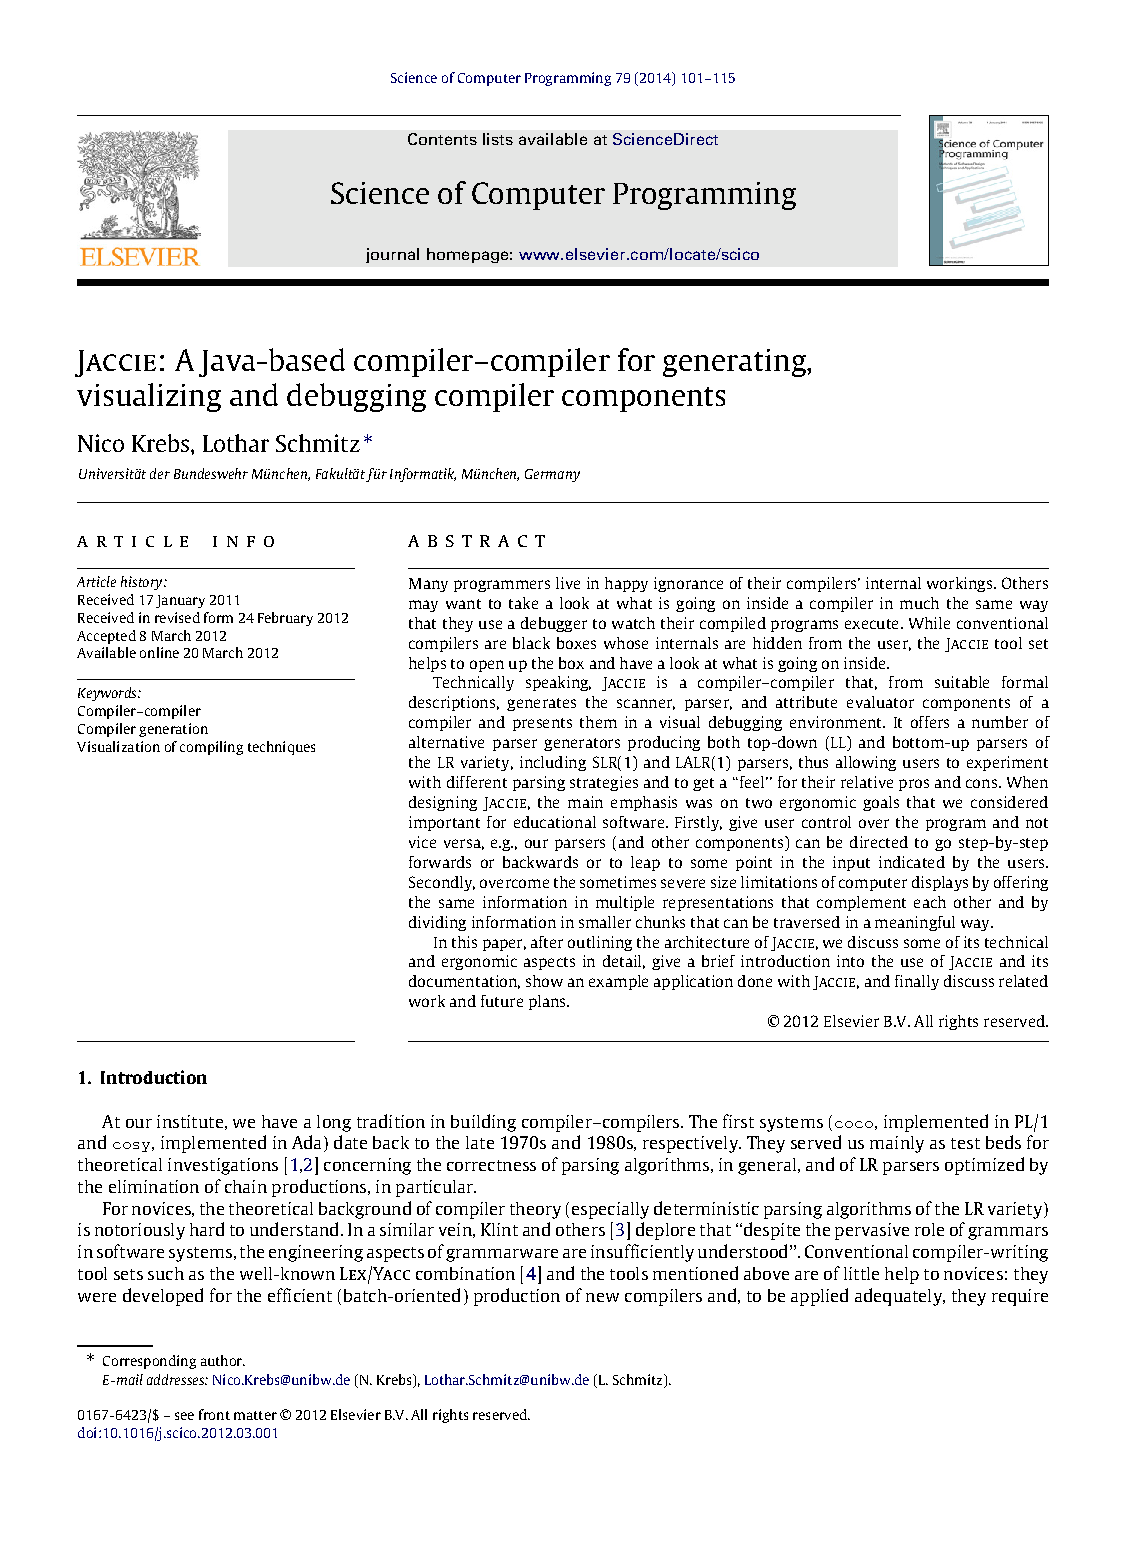
\includepdf[scale=0.8,pages=1,pagecommand=\section{  英文原文}]{jaccie4.pdf}
\includepdf[scale=0.8,pages={2-3,14,15},pagecommand=]{jaccie4.pdf}

% 每个附录单独占一页
\newpage
\section{中文译文}
\centerline{\textbf{\huge{\hei \小三 JACCIE:一个能够生成、可视化、调试编译器组件}}}
\centerline{\textbf{\huge{\hei \小三 基于Java的编译器生成器}}}
\subsection{绪论}
在我们院,我们在构建编译器编译器的悠久传统。第一个系统(COCO,在PL /1日实施
和舒适,在阿达实现)可以追溯到20世纪70年代和80年代后期,分别。他们为我们服务主要是作为测试床的
理论研究[1,2]关于解析算法的正确性,在一般情况下,和LR的解析器通过优化
链制作的消除,尤其如此。

对于新手,​​编译原理的理论背景(的LR品种尤其是确定性的分析算法)
是出了名很难理解。与此类似,陡崖等人[3]痛惜'尽管语法的普遍作用
在软件系统,grammarware工程方面没有得到充分理解'。传统的编译器书写
工具集,如著名的Lex / Yacc的组合[4]和上面提到的工具是帮助不大新手:他们
为高效(面向批处理的)生产的新的编译器进行了开发和,也可以充分应用,但它们需要编译原理的一些现有知识。典型的使用这样的工具集的一些文件的准备开始(S)
描述意源语言的(词汇和上下文无关)语法和可能的翻译的定义
被执行。从这些定义中,工具集,或者产生一个编译器,或者更有可能的错误消息的列表
即,对于非专家,是很难理解并且在采取行动。即使源代码是免费的语法错误和编译器
是成功生成,它可能还没有做什么预期的事情。因此,要找到任何语义错误,测试输入
必须从源语言编写的,并且,施加编译后,它必须被检查是否产生
目标语言文件是否符合预期。如果没有,设置工具提供了追查的原因一点支持
故障。

与此相比,使用嵌入在一个现代的IDE您最喜爱的编程语言的编译器:即使
准备源文件中,有语法高亮的形式互动支持。语法错误不仅上市
由编译器;上的错误消息点击时,一个被带到发生在源代码中的错误是
发现和提供的什么是错的一个(或多或少)有用的指示。对于跟踪语义错误,用户
在执行过程中提供了一个调试工具,使他们能够不断地观察,所谓的手表单元格的值,
即,由用户为此定义表达式。此外,用户还可以通过在任一单步控制执行
程序或具有代码的执行以用户定义的断点打断,如果一些断言(再次定义
由用户)被发现无效。

一个显而易见的想法是同样嵌入编译器编译器的GUI,并提供调试工具,既为找
语法错误和语义错误。这也给新手一个机会,看看是什么里面怎么回事
编译器和开发这样的技术编制有更深的了解。 Jaccie,基于Java的编译器编译器
一个互动的环境,正好被开发用于这一目的。这是自动生成的教育工具
从合适的语言描述和用于在视觉调试执行这些组件编译器组件
环境。调试环境连续显示组件的内部状态,并与控制
鼠标来回移动,在单个或集合的步骤。从源语言描述衍生辅助信息
可以交互查看任意时间。虽然传统的编译器的黑盒子,其内部从隐藏
用户,我们的工具让用户来看看什么是里面发生。

本文的其余部分安排如下。在下一节中,我们列出了两种编译器的基本架构
和编译器编译器。扫描仪和解析器的视觉调试需要保持可见之间的密切关系
扫描器和分析器定义(在正则表达式和上下文无关文法的形式)上,一方面,并​​且,在
另一方面,由扫描仪和解析器个从这些定义衍生使用内部自动机。第3节简要
描述Jaccie如何导​​出'可读'扫描和解析以统一的方式自动机。第4节解释说,真正的
在设计和实施我们的工具的挑战并没有引起理论,而是由世俗符合人体工程学的问题,
他们中的一些电脑显示器的严峻大小的限制引起的。第5节给出了一个介绍Jaccie和
通过讨论它的一些典型屏幕的其功能。我们还描述了哪里Jaccie,其手册和其他有用的
文档可能被发现。第6节描述了从第一作者的作品在UVC采取一个小应用程序(通用
虚拟计算机)的文件长期存档。最后,我们有相关的工作和未来的计划。
\subsection{编译器和编译器生成器的架构}
从概念上讲,编译过程分为三个连续的阶段:在词法分析阶段,扫描仪
组给定的输入文本的字符转换成一个令牌序列。期间的语法分析,语法分析器确定
在语法树的形式此令牌序列的句法结构。在以下的合成阶段,属性评估
被施加到语法树以实现所需翻译结果。例如,一个C编译器将首先确定
在给定的C程序文本标记,然后从该令牌序列构建语法树,并最终产生结果的目标
通过对语法树进行语义动作代码。 (对于编程语言如C,合成阶段通常
落入若干像中间表示生成,优化和目标代码生成子阶段的。
当多元评价子阶段被Jaccie支持,我们这里不涉及这些方面。)

图。 1表示在其右栏中所生成的编译器。从上到下阅读此列中,人们发现这三个
参与翻译编译器组件(扫描仪,分析器,评估)和中间数据(令牌,语法树)
一些输入到翻译过程的结果。在中间栏的编译器编译器连同它的显示
三台发电机。左侧栏表示必须作为输入提供给编译器编译的发电机组件的定义:用于扫描仪发生器,标记定义取正则表达式的形式;上下文无关
语法被输入到解析器发生器;属性定义和属性评估规则必须被添加到每个
上下文无关的生产规则来定义所期望的翻译。当读取从左到右该图中,我们看到,
像在右侧列中所示的编译过程中,某些输入(这里,属性语法定义)是
变换成一个结果(这里,在右手侧上的编译器)。由于这种相似性,在中间设置该工具是
通常被称为编译器编译器,即产生编译器编译器。

在图1,椭圆形和所有程序组件被封闭,所有数据都被长方形框。当读取图
从左至右,所生成的编译器组件(扫描器,解析器,评估器)是数据。当读右手
列从上到下,编译器组件是程序。为了表示这些双重角色,编译器组件
由圆角矩形被封闭。


上面的描述适用于完全相同的方式来生产编译器的编译器一样的Lex/ Yacc的工具集和
到Jaccie。的主要区别在于,莱克斯/ Yacc的通常产生高效黑箱编译器,而内部结构
和由Jaccie生成的编译器的运作能详细在该Jaccie调试编译器运行时被观察到。

在Jaccie工具集,主要部件也对应于图1:每个编译器组件,有一个特殊的
编辑写它的定义,例如,一个直接操纵样式编辑器的上下文无关文法定义解析器。
此外,对于每个编译成分,是用于从定义生成它,然后执行它的组合工具
交互,由用户控制。除了这六个主要工具,有用于观看不少专门的工具
这是由编译器定义的编译器编译器编译而得的信息。

\subsection{在可视化编译器执行的时候}

如在引言中所述,在设计和实施济的真正挑战是不引起理论
但来自两个平凡而符合人体工程学的问题:
\begin{enumerate}
	\item 如何提供足够的用户控制?内鼓励学生做一个模拟环境主动学习
	自己的经验是不是通过基础课程预定顺序步进有效得多[7]。
	因此,主动学习是我们的宗旨。然而,因为翻译过程的性质,主要阶段,词汇
	分析,解析和评价的属性,是必须按照这个顺序基本上是进行确定性的过程。
	尽管如此,Jaccie用户有足够的空间进行实验:
	\begin{itemize}
		\item 用户可以直接扫描的方法中,解析和在他们希望几乎任何方式,例如,Jaccie属性评估
		扫描器可以以单一步骤进行向前和向后,在字符或全令牌单位,或跳跃到一个地方
		在用户点击鼠标的输入。
		\item
		用户可以不同的解析策略之间自由选择:LL(1),LR(0),LR(1),SLR(1),LALR(1),不细致
		这里。
		\item 同样,对于属性的评价不同的策略是提供给用户。一个策略可以让用户直接
		属性评估在运行时(这里是''准备好进行评估'属性'以蓝色显示)。
		\item 所有的时间,通过Jaccie从编译器定义文件所产生的额外信息可以被交互地查看。
		这种信息的例子是第一代/后续集和不同的解析自动派生弗罗马上下文
		语法。
		\item Jaccie解析器的一个重要的调试功能是他们的不确定性分析,例如,SLR(1)语法分析的支持
		非SLR(1)语法。非确定性解析既可以进行自动(探索回溯模式不同的选择),或者由用户直接。该功能是指用于追踪(和消除!)
		非determinism2来源:如果一个解析器是确定性的,它的基本语法是明确的,确保
		对于每个有效的解析器输入恰好有一个句法树,这又是成功属性的前提
		评估。
		\item 最后,JACCIE是一个完整的编译器编译器,使用户能够探索任何定义和投入的机会
		它们可以设想。
	\end{itemize}
	\item 如何应付限制画面大小的问题?即使是小的语法没有电脑显示屏足够大
	提供所有相关信息(属性文法,目前的形势分析,解析自动机,第一代
	/后续套等)在同一时间。显然,现代图形用户界面有点通过提供多种解决这些问题
	对于不同的数据集之间的切换窗口。另外,滚动机制,有助于探索非常大的数据集。为
	上面提到的一些伪影,例如标准窗技术是不够的。因此Jaccie提供
	量身定做的信息更多的机制数量呈现给用户:
	\begin{itemize}
		\item 大语法树不能很好适合于标准滚动机制,因为该图的主要部分
		区往往是空的,并且在一些详细的截面观察时(相当均匀地构建)树结构的用户
		可能会容易丢失。为属性的评价,这得到-丢失效应加剧,因为树的每个节点是
		饰有任何数字携带相关的(有时是广泛的)信息的属性。 一些
		通过Jaccie提供支持方向互补机制是:变焦机构(好相对
		小乔木);用于遍历树的机构(向上或向下)沿着它的结构,或在某些属性的评价
		订购;用于接通和关断特性的细节的机制,包括示出了另一种观点
		当前节点及其全部细节的邻居(包括在这些所有属性依赖的图形表示
		节点)。
		\item LR自动机往往会变得非常大甚至中等规模的上下文无关文法 - 一个国家可以
		随便填的显示。通过所有国家的名单滚动是不是穿越一个自动的一种有意义的方式。 代替,
		Jaccie允许用户通过以下链接遍历自动机的状态。在解析,的当前状态
		解析自动保持可见。行动 - /除了在最后一节中描述的项集,减少了跳转表
		申述,即传统的分析表可用。对于跟踪问题,错误状态的列表给
		立即获得所有包含SHIFT-/ reduce-或减少,冲突的状态。
		\item 
		为LL解析器核心信息(以及与前瞻LR分析器)是所谓的第一代/后续集。 Jaccie不仅
		显示了这些套;它也允许用户从底层上下文无关文法追溯它们的计算。
	\end{itemize}
从本质上讲,所有这些解决方案的两个主题的变化:第一个主题是提供另一种表述,即
相得益彰,给用户一个选择使用什么适合最适合手头解决问题。 第二
主题是随着时间的推移展开大型数据集,并提供有意义的遍历机制。
	

该Jaccie语法编辑器设计,以避免用户错误:它允许每个thename(终端或者非终端)的符号来
在只有一次输入。此后,产生式规则被组装fromthe采用直接操纵组符号,即
拖和下降。这种策略有效地避免了对用户的一部分的任何错别字。符号可能会被重新命名(自动
整个语法一致取代)。此外,可以创建新的符号和现有删除(后者
操作删除符号的所有实例从整个语法)。
修改建议
\end{enumerate}
\subsection{结论:相关工作和未来的计划}
编译器编译器一样Jaccie的理论基础是由唐纳德·E·克努特在他的两个开创性的论文[12铺设,
13]对LR分析和属性语法。编译器和编译器编译器的标准教科书是众所周知的
“'龙书'”[4];作为一个编译器编译器的典型例子,它描述了流行的Lex/ Yacc的系统。

有编译器生成工具军团像Yacc的[14]。事实上,它的名字是“的首字母缩写(选择在1978年!)”不过,
另一个编译器编译器。“生产编译器生成工具”一体的综合性列表(比较themby功能)
维持对Wikipedia.7此列表分为四类:第一包括定期的语言,即扫描程序生成工具;第二类列出的工具确定性上下文无关语言,大部分LALR(1)-parser发电机组;第三类是由'packrat''或递归下降解析器生成的;第四类支持生成更一般的解析技术(如厄雷的[15]或GLR[16]),并往往不区分扫描和解析。对各种分析算法的细节可以在综合教科书[17]中找到。

的“”传统“'从第二类工具的一个优点是一个发电机可以决定所得解析器是否是确定的,因此,会产生一种独特的语法树的每个有效解析器输入。此外,这些工具严格分开的解析器规范和生成的分析器;对递归下降解析器,并且已经成为时下流行的解析器组合,还有就是更换语言规范(即上下文无关文法)语法分析器的代码,甚至更糟糕,用于插入语法树评估代码转换成趋势解析器也是如此。不同相位的这种混合阻碍修改和应,因此,可避免。 LR分析是出了名很难理解为新手,甚至有时专家们可能会发现很难从LALR通过修改它们的基础语法删除不需要的不确定性(1)语法分析器。为了帮助新手和专家克服这些问题,我们已经创建Jaccie:Jaccie的解析器生成,因此,产生确定性(LL(1),LR(0),SLR(1),LALR(1),LR(1))解析器。其扫描,分析,和属性评估阶段是严格分开的。

虽然有很多的编译器生成工具和许多演示工具,可视化的编译过程的某些方面在互联网上被发现,也有相对较少的系统,像Jaccie,旨在传统的编译器生成全面的调试功能相结合。我们都知道只有这种下列系统。

在早期,Ytracc解析浏览系统[18]提出,其Yacc生成自动仪器解析器,以便解析的连续状态在一个文件中被捕获,因为它们进行的。捕获的解析然后可以向前或向后重放,分步实施,或子树子树。观看工具Yshow连续显示解析栈,输入线,其中电流输入令牌突出,由接下来的减少将要进行的规则,命令行的连续五个快照。作者在两个连续的编译器类(各约50人),其中(仪表版本)Ytracc和Yshow则推出多用户Unix环境下自愿使用取得经验的报告;和 - 从由此获得的数据争论 - 他们讨论的细节学生的行为不同的模式。我们自己的类要小得多,学生在自己的私人电脑工作;因此,统计相关的定量数据将很难收集。然而,我们吸取学生如何解决使用Jaccie问题最多。他们的解决方案和意见提供不断改进我们的工具所需要的定性反馈;例如,附带Jaccie的所有例子已经通过一门课程的学员制定出训练演习。

比Ytracc更早和更完整的教育编译器生成,可见归功于翻译系统(VATS),在[19]中描述。像它的前身ATS,它是围绕LL(1)语法分析器生成器内置。相比LALR(1)解析器生成器,所述LL(1)的类型是一般较少(例如,语法不得包含左递归规则),但它融合了嵌入式属性评估越好,因为LL(1)解析器建立较大的语法的部树比其他解析器更快。在解析,ATS-产生的编译器同时评估继承和合成属性。大桶被创造'提供的编译器教程和调试窗口'。在大桶视觉分析器显示输入与由令牌光标标记最近扫描的令牌,同时含有语法和行动码元,并且其中所述分析器的行为被描述消息区解析栈。某些扩展到大桶,即进行“正在开发',称为”有:功能单一步骤的分析算法,以滚动解析栈,以支持回溯和暧昧文法的解析,并显示属性的流值。所有这些功能(及以上)是由Jaccie提供。

最近,商用系统可成为有特色,而类似Jaccie。砂岩公司已销售中所描述的VisualParse++系统[20];它支持LALR解析。解析树或者以三维表示(其中节点被示出为球和由磁极被连接),或在一个2D'堆栈'表示(其允许折叠和展开树),更适合于观看大树可视化。正如所从商业产品可以预料,VisualParse++提供了五个目标语言(C,C++,Java和Delphi和C ++)选择。然而,有没有属性评估发生器:扫描仪发生器只有一个解析器生成的VisualParse++由(像许多其他工具集)。不幸的是,VisualParse++开发似乎已经被抛弃了。

从马里博尔大学与国际合作伙伴共同的一个研究小组已经开发出了LISA [21]的系统,其列表的功能非常相似Jaccie的:有一个数字解析器生成的,属性评估发电机,和可视化工具。此外,LISA支持面向方面的执行编译组件。在首页上的LISA工具可以下载作为一个Java JAR文件。通过运行该工具,但细节不能被检查合适的文档想:该工具的联机帮助说,'在线帮助尚不可用'并指向LISA主页以获取更多信息。在那里,在参考手册,另一个指针''对于图形模式的IDE看看教程的工具演示部分采用LISA'引导读者的PDF文档,其中包含了一系列的注释截图,在没有办法足以解释LISA的图形用户界面,特别是,它的许多选项。该网页一直没有更新了五年,这显然是事实不完全显示,丽莎的发展已经被抛弃了。


更近期,Hielscher和Wagenknecht创建的工具集AtoCC8:用于生成和可视化编译器组件松散连接工具的集合。为了演示一个特别好的特性是有限自动机不仅可以直观地编辑,但也可以是动态的。 (类似的说明也适用于关于vLex工具[22],其中详细可视化从正则表达式扫描自动机的标准偏差,以及LL的视觉结构(1)和所示SLR(1)与JFLAP9演示工具解析器,在JFLAP教程)。AtoCC还提供了定义扫描仪和分析器独立的可视化编辑器。同样地,T型图(如由尼克劳斯·维尔特引入)可以在视觉上编辑和产生的。然而,象对VisualParse++没有属性评估发生器。

流行的ANTLR(另一个工具语言识别)工具set10使用扩展LL(k)的解析技术作为一种更自然的替代LALR(1)分析。尽管如此,由播威和帕尔在[23]指出,ANTLR用户需要通过解决分析器非确定性的来源支持这些复杂的开发环境。这种支持是由ANTLR的-作品,视觉前端的ANTLR工具提供。 “他们承认在改变显示器的输入流,解析器超前,解析树,解析堆栈和AST的'的AntlrWorks调试器通过套接字机制和”连接到ANTLR“。语法图的窗口,非确定性被显示为高亮暧昧路径语法开发商。然而,AntlrWorks和ANTLR是针对未使用其他工具集的特殊的分析策略。

从众多工具集,提供更多的基本的可视化和调试功能,我们只提JS / CC,11的LALR(1)使用JavaScript同时作为实施和目标语言,也解析器生成提供了一个''在线直播安装''的在线测试。

综上,我们认为,在目前可用的语法工具集先河,功能Jaccie的组合 - 一个完整的编译器编译器包括替代(LL和LR风格)分析器发电机和属性评估,再加上可视化组件过多,所有顺利地集成到一个统一的调试环境和全面的文件,包括许多已经解决的例子 - 是独一无二的。

不过,有一个'愿望清单'的功能,这将有助于进一步提高Jackie和我们打算在未来的版本包括:
\begin{itemize}
	\item 在外部渲染与Graphviz的12点自动格式和语法树输出;同样,XML输出以及与其他工具进行数据交换输入;
	\item 产生错误处理程序的支持;这是用于解析特别重要,但将其他组件的一个有用的扩展为好;
	\item 生成编译器组件不仅在Java中,而且在其他目标语言的源代码灵活的支持;这将允许用户生成的编译器组件集成到自己的软件;
	\item 提供更先进的,高效的属性评估策略,例如,对奥克斯的支持(有序属性文法)在[24]中定义。
\end{itemize}

\end{document}

